\section{Les suites}
\subsection{Les suites arithmétiques}
\begin{definition}
    Soit $(u_n)_{n\in\mathbb{N}}$ une suite. On dit que $(u_n)$ est une \emph{suite arithmétique} si et seulement si $\exists r\in\mathbb{R} : \forall n\in\mathbb{N}, u_{n+1}-u_n=r$. Dans ce cas, on appelle $r$ la \emph{raison} de la suite.
\end{definition}
\begin{propriete}
    Soit $(u_n)_{n\in\mathbb{N}}$ une suite arithmétique de raison $r$. On a :
    $$\forall n\in\mathbb{N}, u_n=u_0+nr$$
\end{propriete}
\begin{propriete}
    Soit $(u_n)_{n\in\mathbb{N}}$ une suite arithmétique de raison $r$. On a :
    $$\forall n,p\in\mathbb{N} : p\leq n, u_n=u_p+(n-p)r$$
\end{propriete}
\subsubsection{Monotonie}
\begin{propriete}
    Soit $(u_n)_{n\in\mathbb{N}}$ une suite arithmétique de raison $r$ non nulle.
    $$\begin{cases}
        r>0 & (u_n) ~\text{est croissante}\\
        r<0 & (u_n) ~ \text{est décroissante}
    \end{cases}$$
\end{propriete}
\subsubsection{Somme de termes consécutifs}
La somme des $n$ termes consécutifs d'une suite arithmétique est donnée par la formule :
$$
S_n = \frac{n+1}{2} \cdot (a_0 + a_n)
$$

où $S_n$ est la somme des $n+1$ termes, $a_0$ est le premier terme, $a_n$ est le dernier terme et $n+1$ est le nombre de termes.

\subsection{Les suites géométrique}
\begin{definition}
    Soit $(u_n)_{n\in\mathbb{N}}$ une suite non nulle. On dit que $(u_n)$ est une \emph{suite géométrique} si et seulement si $\exists r\in\mathbb{R}^* : \forall n\in\mathbb{N}, \frac{u_{n+1}}{u_n}=q$. Dans ce cas, on appelle $q$ la \emph{raison} de la suite.
\end{definition}
\begin{propriete}
    Soit $(u_n)_{n\in\mathbb{N}}$ une suite géométrique de raison $q$. On a :
    $$\forall n\in\mathbb{N}, u_n=u_0*q^n$$
\end{propriete}
\begin{propriete}
    Soit $(u_n)_{n\in\mathbb{N}}$ une suite géométrique de raison $q$. On a :
    $$\forall n,p\in\mathbb{N} : p\leq n, u_n=u_p*q^{(n-p)}$$
\end{propriete}
\subsubsection{Monotonie}
\begin{propriete}
    Soit $(u_n)_{n\in\mathbb{N}}$ une suite géométrique de raison $q$ non nulle.\\
    Si $u_0$ est positif:
    $$\begin{cases}
        q>1 & (u_n) ~\text{est croissante}\\
        0<q<1 & (u_n) ~ \text{est décroissante}
    \end{cases}$$
    Si $u_0$ est négatif:
    $$\begin{cases}
        q>1 & (u_n) ~\text{est décroissante}\\
        0<q<1 & (u_n) ~ \text{est croissante}
    \end{cases}$$
\end{propriete}décroissante
\begin{propriete}
    Soit $(u_n)_{n\in\mathbb{N}}$ une suite géométrique de raison $q$ non nulle.\\
    $$\begin{cases}
        |q|>1 & (u_n) ~\text{est divergente}\\
        0<|q|<1 & (u_n) ~ \text{est convergente}\\
        q=1 & (u_n) ~\text{est constante}\\
        q=-1 & (u_n) ~\text{oscille entre}~u_0 ~\text{et}~ u_1
    \end{cases}$$
\end{propriete}
\subsubsection{Exemples graphiques}

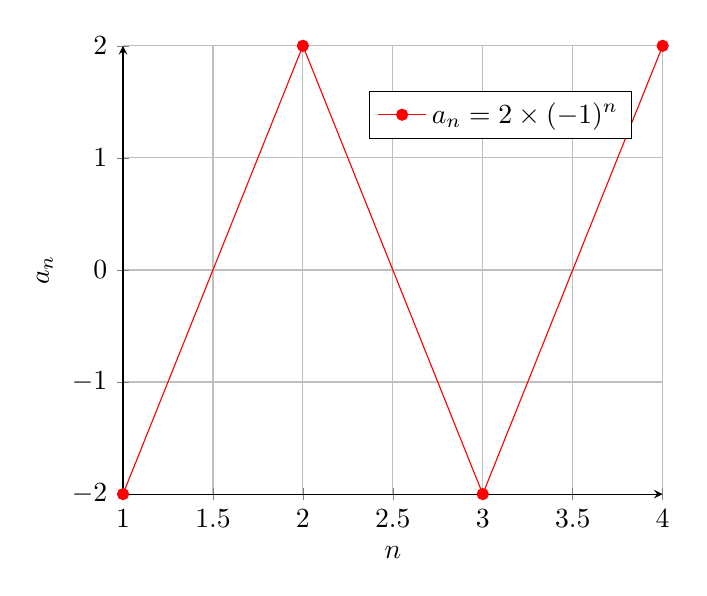
\begin{tikzpicture}
  \begin{axis}[
    xlabel={$n$},
    ylabel={$a_n$},
    axis lines=left,
    grid,
    mark=*,
    legend style={at={(0.7,0.9)},anchor=north}
  ]

  % Définition de la suite oscillante
  \def\a{2}
  \def\r{-1}
  
  % Calcul des premiers termes
  \pgfmathsetmacro{\aOne}{-\a}
  \pgfmathsetmacro{\aTwo}{\a}
  \pgfmathsetmacro{\aThree}{-\a}
  \pgfmathsetmacro{\aFour}{\a}

  % Tracé des points
  \addplot[red, mark=*] coordinates {(1, \aOne) (2, \aTwo) (3, \aThree) (4, \aFour)};
  \addlegendentry{$a_n = 2 \times (-1)^{n}$}

  \end{axis}
\end{tikzpicture}
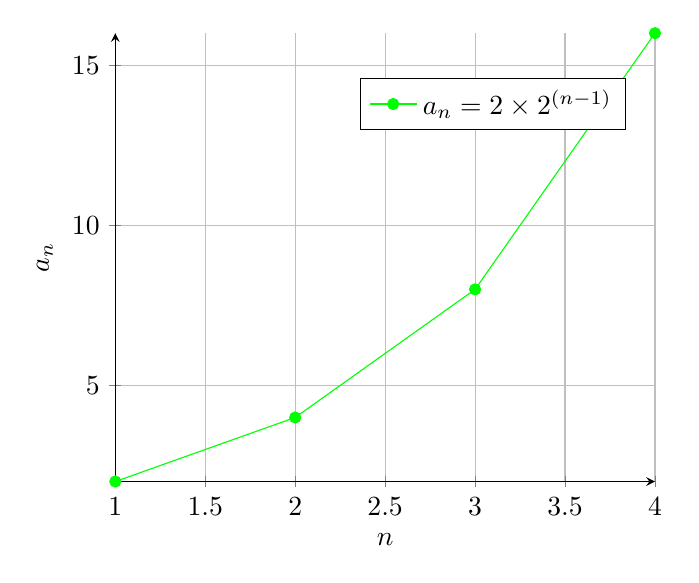
\begin{tikzpicture}
  \begin{axis}[
    xlabel={$n$},
    ylabel={$a_n$},
    axis lines=left,
    grid,
    mark=*,
    legend style={at={(0.7,0.9)},anchor=north}
  ]

  % Définition de la suite géométrique divergente
  \def\a{2}
  \def\r{2}
  
  % Calcul des premiers termes
  \pgfmathsetmacro{\aOne}{\a * \r^0}
  \pgfmathsetmacro{\aTwo}{\a * \r^1}
  \pgfmathsetmacro{\aThree}{\a * \r^2}
  \pgfmathsetmacro{\aFour}{\a * \r^3}

  % Tracé des points
  \addplot[green, mark=*] coordinates {(1, \aOne) (2, \aTwo) (3, \aThree) (4, \aFour)};
  \addlegendentry{$a_n = 2 \times 2^{(n-1)}$}

  \end{axis}
\end{tikzpicture}
\\[0.5cm]
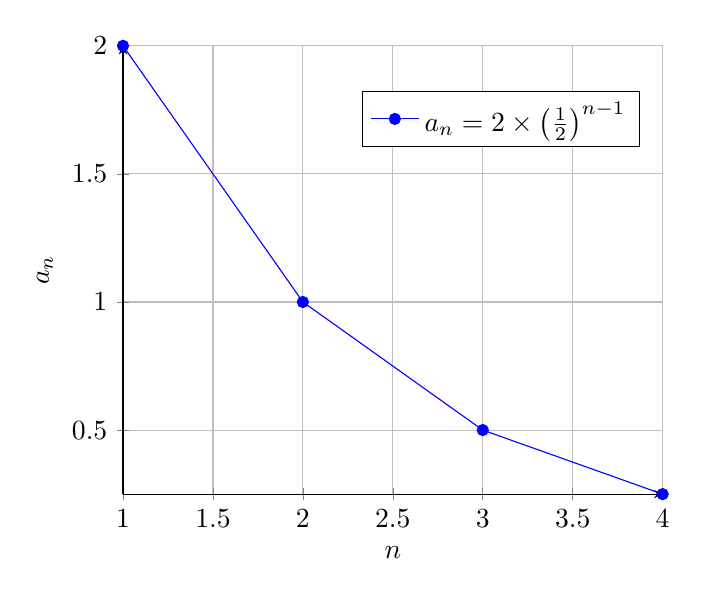
\begin{tikzpicture}
  \begin{axis}[
    xlabel={$n$},
    ylabel={$a_n$},
    axis lines=left,
    grid,
    mark=*,
    legend style={at={(0.7,0.9)},anchor=north}
  ]

  % Définition de la suite géométrique convergente
  \def\a{2}
  \def\r{0.5}
  
  % Calcul des premiers termes
  \pgfmathsetmacro{\aOne}{\a * \r^0}
  \pgfmathsetmacro{\aTwo}{\a * \r^1}
  \pgfmathsetmacro{\aThree}{\a * \r^2}
  \pgfmathsetmacro{\aFour}{\a * \r^3}

  % Tracé des points
  \addplot[blue, mark=*] coordinates {(1, \aOne) (2, \aTwo) (3, \aThree) (4, \aFour)};
  \addlegendentry{$a_n = 2 \times \left(\frac{1}{2}\right)^{n-1}$}

  \end{axis}
\end{tikzpicture}
\subsubsection{Somme de n termes consécutifs}
La somme de $n$ termes consécutifs d'une suite géométrique est donnée par la formule :
$$
\begin{cases}
    S_n = a_1 \cdot \frac{q^n - 1}{q - 1} & \text{si}~q\ne 1\\
    S_n =n\cdot a_1 & \text{sinon}
\end{cases}
$$
où\\
\begin{center}
    \begin{minipage}{0.4\textwidth}
    \begin{itemize}
    \item $S_n$ est la somme des $n$ termes consécutifs
    \item $a_1$ est le premier terme
    \end{itemize}
\end{minipage}
\begin{minipage}{0.4\textwidth}
    \begin{itemize}
    \item $r$ est la raison de la suite géométrique
    \item $n$ est le nombre de termes
    \end{itemize}
\end{minipage}
\end{center}
\newpage
\subsection{Récapitulatif sur les suites}
\begin{codeb}
    

\begin{enumerate}
    \item Une suite $\left(u_n\right)$ peut être définie de façon explicite : il existe alors une fonction $f$ définie sur $D_f$ telle que, pour tout entier $n \in D_f, u_n=f(n)$. Cela permet de:
    \begin{itemize}
        \flch modéliser une situation qui dépend de $n$;
        \flch calculer un terme quelconque de la suite en lien avec la situation.
    \end{itemize}
    \item Une suite $\left(u_n\right)$ à valeurs dans $\mathcal{D}_m$ peut être définie par récurrence : il existe alors une fonction $g$ définie sur $D_g$ telle que, pour tout $n \in \mathbb{N}, u_{n+1}=g\left(u_n\right)$. Cela permet de :
    \begin{itemize}
        \flch modéliser une situation dans laquelle un terme dépend du précédent.
    \end{itemize}
    \item $\left(u_n\right)$ est croissante à partir de $n=0$ lorsque, pour tout $n \in \mathbb{N}, u_{n+1} \geqslant u_n$ et $\left(u_n\right)$ est décroissante à partir de $n=0$ lorsque, pour tout $n \in \mathbb{N}, u_{n+1}\leq u_n$. Cela permet de:
    \begin{itemize}
        \flch trouver le sens de variation d'une suite;
        \flch résoudre des problèmes liés à des situations de variations.
    \end{itemize}
    \item Une suite est arithmétique lorsqu'il existe un réel $r$ tel que, pour tout $n \in \mathbb{N}, u_{n+1}=u_n+r$.
    
    Pour tous entiers naturels $n$ et $p, u_n=u_p+(n-p)\times r$ et, en particulier, $u_n=u_0+n r$.
    
    Une suite arithmétique de raison $r$ est croissante si $r>0$, décroissante si $r<0$ et constante si $r=0$.
    
    Pour tout entier naturel $n$ non nul, $1+2+\ldots+n=\frac{n(n+1)}{2}$. Cela permet :
    \begin{itemize}
        \flch étudier une situation de récurrence où un terme s'obtient à partir du précédent en ajoutant toujours le même nombre.
    \end{itemize}
\end{enumerate}
\end{codeb}


